% Created 2024-07-23 Tue 14:14
% Intended LaTeX compiler: lualatex
\documentclass[presentation,professionalfonts,smaller,aspectratio=169]{beamer}
                


\makeatletter
 \@ifclassloaded{beamer}{%
  %%% save beamer's `solution' environment as `beamersolution':
  \let\beamersolution\solution
  \let\endbeamersolution\endsolution
  %%% "delete" the `solution' environment:
  \let\solution\relax
  \let\endsolution\relax
}{%
}%
\makeatother
\usepackage[utf8]{inputenc}
\usepackage[T1]{fontenc}
%\usepackage[french]{babel}
\usepackage[portuguese]{babel}

%%%% FONTS




\usepackage{xsim}
\usepackage[most]{tcolorbox}
\usepackage{amssymb}
\usepackage{fontawesome}
\newcounter{paragraph}



\DeclareExerciseEnvironmentTemplate{custom}{%
  \begin{tcolorbox}[boxrule = 0pt]
  \tcbox[on line,colback=teal,colframe=teal,coltext=white,size=small]{%
    \faBook\sffamily\bfseries\
    \XSIMmixedcase{\GetExerciseName}
    \GetExerciseProperty{counter}%
  }\quad
}{\end{tcolorbox}}


\DeclareExerciseEnvironmentTemplate{custom2}{%
  \begin{tcolorbox}[boxrule = 0pt]
  \tcbox[on line,colback=violet,colframe=violet,coltext=white,size=small]{%
    \faToggleOn\sffamily\bfseries\
    \XSIMmixedcase{\GetExerciseName}
    \GetExerciseProperty{counter}%
  }\quad
}{\end{tcolorbox}}




\DeclareExerciseType{test}{
	exercise-env = question ,
	solution-env = answer ,
	exercise-template = custom ,
	solution-template = custom2 ,
	exercise-name	= Exemplo. ,
	exercises-name = Exemplo ,
	solution-name = Solução ,
	solutions-name = Sol. ,
	exercise-heading = \textbf ,
	solution-heading = \textbf
}


\xsimsetup{
  exercise/within = section,
  exercise/the-counter =  \arabic{exercise}, 
%%solution-name = solution,  % used with headings=true
solution/print=false,
%print-collection/print=both,
}





\usepackage{colortbl}
\usepackage[tikz]{bclogo}
\usetikzlibrary{fit,patterns,shadows.blur,shapes,mindmap}
\usetikzlibrary{arrows,calc,arrows.meta,decorations.markings,shapes.symbols}
\usetikzlibrary{decorations.pathreplacing, decorations.pathmorphing,calc,arrows,positioning}
\usepackage{tikzpeople}
\usepackage{qrcode,hyperref}
\usepackage{upgreek}
%\usepackage[version=4]{mhchem}
\usepackage{tabularray}


\NewTblrTheme{fancy}{
\SetTblrStyle{caption-tag}{font=\bfseries}
\SetTblrInner[tblr,longtblr]{rowsep=2.5pt}
\DefTblrTemplate{firsthead, middlehead,lasthead}{default}{} % <---
\DefTblrTemplate{contfoot-text}{normal}{\scriptsize\textit{Continued on the next page}}
\SetTblrTemplate{contfoot-text}{normal}
}






\usepackage{chemfig,chemmacros,elements,chemformula}
\chemsetup{modules={all}}
\chemsetup[redox]{pos=top,roman=false}
\chemsetup[redox]{pos=top}
\chemsetup{redox/sep=.5em}
\chemsetup[redox]{explicit-sign=true}
\NewChemPhase\lqdd{\(\ell\)}
\NewChemPhase\gr{grafite}
\NewChemPhase\reac{reação}
\NewChemState\Enthalpy{symbol=H,superscript=,unit=\kilo\joule}%
\usepackage{siunitx}
\setchemfig{fixed length=false, atom sep=2.5em, arrow offset=6pt, scheme debug=false}%,angle increment=30}
\renewcommand*\printatom[1]{\ensuremath{\mathsf{#1}}} % This line changes the font of the atoms to sans serif
%%%% QRCODE
\usepackage{pdfpages}
\usepackage{mol2chemfig}
\usepackage{subfig,caption}
\usepackage{wrapfig}
\usepackage{enumitem}
\setitemize{label=\usebeamerfont*{itemize item}%
\usebeamercolor[fg]{itemize item}
\usebeamertemplate {itemize item}}
\usepackage{array} % ajust colunm table
\usepackage{cancel}
\usepackage[controls]{animate}
\renewcommand{\CancelColor}{\color{red}}

%%%%%%%%%%%%%%%%%%% CONFIG TCOLORBOX 

\newtcolorbox{mybox}[2][]{boxsep=0.5em,left=0.5em,
colback=blue!5!white, colframe=blue!75!black,
fonttitle=\bfseries\sffamily,
colbacktitle=blue!85!red!60,enhanced,
attach boxed title to top left={yshift=-3mm,xshift=5mm},
title=#2,#1}

\newtcolorbox{myrule}[2][]{boxsep=0.5em,left=0.5em,
colback=green!5!white, colframe=blue!75!black,
fonttitle=\bfseries\sffamily,
colbacktitle=blue!85!red!60,enhanced,
attach boxed title to top left={yshift=-3mm,xshift=5mm},
title=#2,#1}


\newtcolorbox{myex}[2][]{boxsep=0.5em,left=0.5em,
  colback=yellow!5!white, colframe=blue!75!black, 
  fonttitle=\bfseries\sffamily,
  colbacktitle=blue!85!red!60,enhanced,
  attach boxed title to top left={yshift=-3mm,xshift=5mm},
  title=#2,#1}


 \definecolor{col1}{HTML}{FF7878}
 \definecolor{col2}{HTML}{51B5F8}
 \definecolor{col3}{HTML}{68E1AA}
 \definecolor{col4}{HTML}{B869EA}
 \definecolor{col5}{HTML}{FF5500}
 \definecolor{col6}{HTML}{FFF8E7}
 \definecolor{col7}{HTML}{FF9966}
 \definecolor{col8}{HTML}{9400D3}



\definesubmol\nobond{-[,0.2,,,draw=none]\scriptstyle\color{blue}}
\newcommand{\re}{\hspace{-1cm}}
\newcommand{\af}{\hspace{2cm}}

\date{}
% \usetheme{minflat}
\DeclareExerciseCollection{Hidro}
\usetheme{minflat}
\author{Fábio Lima}
\date{}
\title{Hidrocarbonetos Não Ramificados}
\hypersetup{
 pdfauthor={Fábio Lima},
 pdftitle={Hidrocarbonetos Não Ramificados},
 pdfkeywords={},
 pdfsubject={},
 pdfcreator={Emacs 29.4 (Org mode 9.6.15)}, 
 pdflang={En Portuguese}}
\begin{document}

\maketitle
\begin{frame}{Outline}
\tableofcontents
\end{frame}




\section{Hidrocarbonetos}
\label{sec:orgd259638}
\begin{frame}[label={sec:orgb4105b0}]{Hidrocarbonetos}
São compostos orgânicos formados exclusivamente por átomos de carbono e de hidrogênio.
%\relax 
\providecommand\zref@newlabel[2]{}
\providecommand\hyper@newdestlabel[2]{}
\@setckpt{../img/diagrama}{
\setcounter{page}{4}
\setcounter{equation}{0}
\setcounter{enumi}{0}
\setcounter{enumii}{0}
\setcounter{enumiii}{0}
\setcounter{enumiv}{0}
\setcounter{footnote}{0}
\setcounter{mpfootnote}{0}
\setcounter{beamerpauses}{1}
\setcounter{section@level}{0}
\setcounter{bookmark@seq@number}{1}
\setcounter{lecture}{0}
\setcounter{part}{0}
\setcounter{section}{1}
\setcounter{subsection}{0}
\setcounter{subsubsection}{0}
\setcounter{subsectionslide}{2}
\setcounter{framenumber}{4}
\setcounter{figure}{0}
\setcounter{table}{0}
\setcounter{parentequation}{0}
\setcounter{theorem}{0}
\setcounter{LT@tables}{0}
\setcounter{LT@chunks}{0}
\setcounter{r@tfl@t}{0}
\setcounter{mdf@globalstyle@cnt}{1}
\setcounter{mdfcountframes}{0}
\setcounter{mdf@env@i}{0}
\setcounter{mdf@env@ii}{0}
\setcounter{mdf@zref@counter}{0}
\setcounter{bclogocompteur}{0}
\setcounter{qr@i}{254}
\setcounter{qr@j}{0}
\setcounter{maski}{0}
\setcounter{maskj}{0}
\setcounter{totalones}{0}
\setcounter{penaltyi}{0}
\setcounter{penaltyii}{0}
\setcounter{penaltyiii}{0}
\setcounter{penaltyiv}{0}
\setcounter{qr@hexchars}{0}
\setcounter{qr@divisionsremaining}{0}
\setcounter{@elements@orbital@type}{0}
\setcounter{@elements@shell@number}{0}
\setcounter{reaction}{0}
\setcounter{cmpdmain}{0}
\setcounter{AM@survey}{0}
\setcounter{caption@flags}{0}
\setcounter{continuedfloat}{0}
\setcounter{KVtest}{0}
\setcounter{subfigure}{0}
\setcounter{subfigure@save}{0}
\setcounter{depth}{1}
\setcounter{subtable}{0}
\setcounter{subtable@save}{0}
\setcounter{@anim@ltxcnt}{0}
\setcounter{tcbbreakpart}{0}
\setcounter{tcblayer}{0}
\setcounter{tcolorbox@number}{0}
\setcounter{tcbrastercolumn}{1}
\setcounter{tcbrasterrow}{1}
\setcounter{tcbrasternum}{1}
\setcounter{tcbraster}{0}
\setcounter{lstnumber}{1}
\setcounter{tcblisting}{0}
\setcounter{tcb@cnt@boxex}{0}
\setcounter{mycounter}{0}
\setcounter{sectionsCounter}{1}
\setcounter{progressBarCounter}{0}
\setcounter{scheme}{0}
\setcounter{lstlisting}{0}
}

\end{frame}



\begin{frame}[label={sec:orgdbf5b60}]{Hidrocarbonetos}
\begin{itemize}
\item Podem ser obtidos a partir da destilação fracionada do petróleo. Esquema de uma torre de fracionamento.
\end{itemize}

\begin{figure}[htbp]
\centering
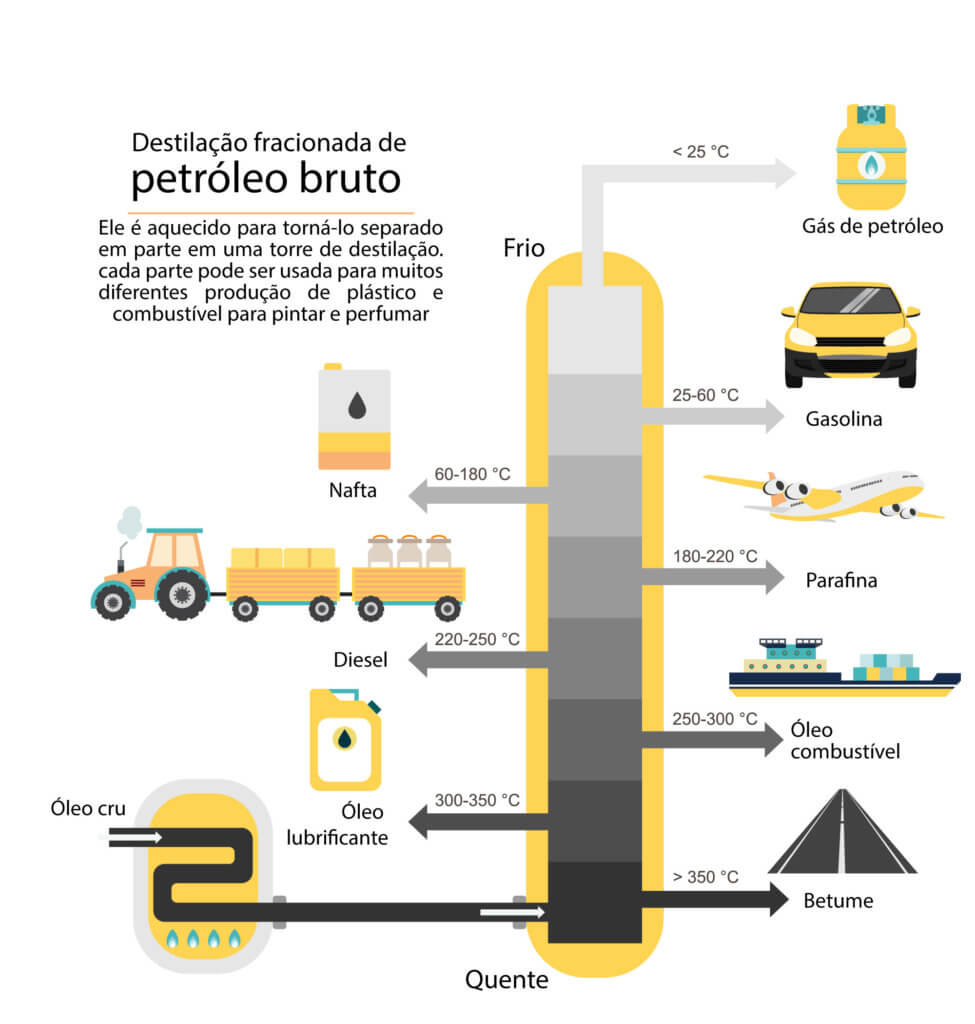
\includegraphics[width=0.4\textwidth]{QO/Hidrocarbonetos/torre.jpg}
\caption{\label{fig:org3022ad4}Esquema de uma torre de fracionamento.}
\end{figure}
\end{frame}

\begin{frame}[label={sec:org8337f74}]{Frações Típicas do Petróleo}
\begin{tabular}{|B|B|B|L|}
\hline
 \cellcolor{green!20} {\bfseries Fração}   &  \cellcolor{green!20} {\bfseries T. de Ebulição (°C)}   &  \cellcolor{green!20} {\bfseries Composição aproximada}  &  \cellcolor{green!20} {\bfseries Usos} \\[0pt]
\hline
Gás residual & - &  \ch{C1-C2} & gás combustível\\[0pt]
\hline
Gás liquefeito de petróleo - GLP & Até 40 &  \ch{C3-C4}  & gás combustível engarrafado, uso doméstico e indrustrial\\[0pt]
\hline
Gasolina & 40-175 & \ch{C5-C10} & combustível de automóveis, solvente\\[0pt]
\hline
Querosene & 175-235 & \ch{C11-C12} & iluminação, combustível de aviões a jato\\[0pt]
\hline
Gasoléo leve & 235-305 & \ch{C13-C17} & diesel, fornos\\[0pt]
\hline
Gasoléo pesado & 305-400 & \ch{C18-C25} & combustível, matéria-prima para lubrificantes\\[0pt]
\hline
Lubrificantes & 400-510 & \ch{C26-C38} & óleos librificantes\\[0pt]
\hline
Resíduo & Acima de 510 & \ch{C38-} & asfalto, piche, impermeabilizantes\\[0pt]
\hline
\end{tabular}
\end{frame}


\section{Classificação}
\label{sec:org2158f47}

\begin{frame}[label={sec:org1d919c1}]{Grupos}
\begin{itemize}
\item Os nomes \emph{alcanos}, \emph{alcenos}, \emph{alcinos}, \emph{alcadienos} \emph{ciclanos}, \emph{ciclenos} e \emph{aromáticos} designam grupos aos quais os hidrocarbonetos pertencem
\end{itemize}



\tikzset{every picture/.style={line width=0.75pt}} %set default line width to 0.75pt        

\begin{tikzpicture}[x=0.75pt,y=0.75pt,yscale=-.8,xscale=.8]
	%uncomment if require: \path (0,322); %set diagram left start at 0, and has height of 322
	
	%Rounded Rect [id:dp08223711771224063] 
	\draw  [color={rgb, 255:red, 80; green, 227; blue, 194 }  ,draw opacity=1 ][fill={rgb, 255:red, 148; green, 243; blue, 222 }  ,fill opacity=1 ] (61.13,74.87) .. controls (61.13,69.12) and (65.79,64.47) .. (71.53,64.47) -- (180.27,64.47) .. controls (186.01,64.47) and (190.67,69.12) .. (190.67,74.87) -- (190.67,106.07) .. controls (190.67,111.81) and (186.01,116.47) .. (180.27,116.47) -- (71.53,116.47) .. controls (65.79,116.47) and (61.13,111.81) .. (61.13,106.07) -- cycle ;
	
	%Rounded Rect [id:dp6837192782695966] 
	\draw  [color={rgb, 255:red, 80; green, 227; blue, 194 }  ,draw opacity=1 ][fill={rgb, 255:red, 148; green, 243; blue, 222 }  ,fill opacity=1 ] (61,199.89) .. controls (61,194.43) and (65.43,190) .. (70.89,190) -- (180.77,190) .. controls (186.24,190) and (190.67,194.43) .. (190.67,199.89) -- (190.67,229.57) .. controls (190.67,235.04) and (186.24,239.47) .. (180.77,239.47) -- (70.89,239.47) .. controls (65.43,239.47) and (61,235.04) .. (61,229.57) -- cycle ;
	
	%Straight Lines [id:da6268575897929107] 
	\draw    (191.05,90) -- (216.63,90) -- (229.05,90) ;
	%Straight Lines [id:da3912391218322656] 
	\draw    (190.55,215) -- (229.97,214.65) ;
	%Straight Lines [id:da4298017873828953] 
	\draw    (229.55,41) -- (229.55,150) ;
	%Straight Lines [id:da4620664162425595] 
	\draw    (229.55,41) -- (264.55,41) ;
	\draw [shift={(266.55,41)}, rotate = 180] [color={rgb, 255:red, 0; green, 0; blue, 0 }  ][line width=0.75]    (10.93,-3.29) .. controls (6.95,-1.4) and (3.31,-0.3) .. (0,0) .. controls (3.31,0.3) and (6.95,1.4) .. (10.93,3.29)   ;
	%Straight Lines [id:da6877154695298078] 
	\draw    (229.55,78) -- (264.55,78) ;
	\draw [shift={(266.55,78)}, rotate = 180] [color={rgb, 255:red, 0; green, 0; blue, 0 }  ][line width=0.75]    (10.93,-3.29) .. controls (6.95,-1.4) and (3.31,-0.3) .. (0,0) .. controls (3.31,0.3) and (6.95,1.4) .. (10.93,3.29)   ;
	%Straight Lines [id:da7148044014610523] 
	\draw    (229.55,113) -- (264.55,113) ;
	\draw [shift={(266.55,113)}, rotate = 180] [color={rgb, 255:red, 0; green, 0; blue, 0 }  ][line width=0.75]    (10.93,-3.29) .. controls (6.95,-1.4) and (3.31,-0.3) .. (0,0) .. controls (3.31,0.3) and (6.95,1.4) .. (10.93,3.29)   ;
	%Straight Lines [id:da2252897061575344] 
	\draw    (229.55,150) -- (264.55,150) ;
	\draw [shift={(266.55,150)}, rotate = 180] [color={rgb, 255:red, 0; green, 0; blue, 0 }  ][line width=0.75]    (10.93,-3.29) .. controls (6.95,-1.4) and (3.31,-0.3) .. (0,0) .. controls (3.31,0.3) and (6.95,1.4) .. (10.93,3.29)   ;
	%Shape: Ellipse [id:dp7986791667582457] 
	\draw  [color={rgb, 255:red, 247; green, 226; blue, 226 }  ,draw opacity=1 ][fill={rgb, 255:red, 247; green, 226; blue, 226 }  ,fill opacity=1 ] (272.8,41.9) .. controls (272.8,34.11) and (278.68,27.8) .. (285.93,27.8) .. controls (293.19,27.8) and (299.07,34.11) .. (299.07,41.9) .. controls (299.07,49.69) and (293.19,56) .. (285.93,56) .. controls (278.68,56) and (272.8,49.69) .. (272.8,41.9) -- cycle ;
	%Shape: Ellipse [id:dp6720086785512882] 
	\draw  [color={rgb, 255:red, 247; green, 226; blue, 226 }  ,draw opacity=1 ][fill={rgb, 255:red, 247; green, 226; blue, 226 }  ,fill opacity=1 ] (273.6,77.1) .. controls (273.6,69.31) and (279.48,63) .. (286.73,63) .. controls (293.99,63) and (299.87,69.31) .. (299.87,77.1) .. controls (299.87,84.89) and (293.99,91.2) .. (286.73,91.2) .. controls (279.48,91.2) and (273.6,84.89) .. (273.6,77.1) -- cycle ;
	%Shape: Ellipse [id:dp15012520451579814] 
	\draw  [color={rgb, 255:red, 247; green, 226; blue, 226 }  ,draw opacity=1 ][fill={rgb, 255:red, 247; green, 226; blue, 226 }  ,fill opacity=1 ] (272.8,113.7) .. controls (272.8,105.91) and (278.68,99.6) .. (285.93,99.6) .. controls (293.19,99.6) and (299.07,105.91) .. (299.07,113.7) .. controls (299.07,121.49) and (293.19,127.8) .. (285.93,127.8) .. controls (278.68,127.8) and (272.8,121.49) .. (272.8,113.7) -- cycle ;
	%Shape: Ellipse [id:dp5861118582212286] 
	\draw  [color={rgb, 255:red, 247; green, 226; blue, 226 }  ,draw opacity=1 ][fill={rgb, 255:red, 247; green, 226; blue, 226 }  ,fill opacity=1 ] (274.4,146.7) .. controls (274.4,138.91) and (280.28,132.6) .. (287.53,132.6) .. controls (294.79,132.6) and (300.67,138.91) .. (300.67,146.7) .. controls (300.67,154.49) and (294.79,160.8) .. (287.53,160.8) .. controls (280.28,160.8) and (274.4,154.49) .. (274.4,146.7) -- cycle ;
	%Straight Lines [id:da04862363537332304] 
	\draw    (229.47,189.65) -- (230.47,249.65) ;
	%Straight Lines [id:da5215534876730717] 
	\draw    (229.55,190) -- (264.55,190) ;
	\draw [shift={(266.55,190)}, rotate = 180] [color={rgb, 255:red, 0; green, 0; blue, 0 }  ][line width=0.75]    (10.93,-3.29) .. controls (6.95,-1.4) and (3.31,-0.3) .. (0,0) .. controls (3.31,0.3) and (6.95,1.4) .. (10.93,3.29)   ;
	%Straight Lines [id:da4160518205492374] 
	\draw    (230.47,249.65) -- (265.47,249.65) ;
	\draw [shift={(267.47,249.65)}, rotate = 180] [color={rgb, 255:red, 0; green, 0; blue, 0 }  ][line width=0.75]    (10.93,-3.29) .. controls (6.95,-1.4) and (3.31,-0.3) .. (0,0) .. controls (3.31,0.3) and (6.95,1.4) .. (10.93,3.29)   ;
	%Shape: Ellipse [id:dp4727286644743499] 
	\draw  [color={rgb, 255:red, 247; green, 226; blue, 226 }  ,draw opacity=1 ][fill={rgb, 255:red, 247; green, 226; blue, 226 }  ,fill opacity=1 ] (273.8,190.9) .. controls (273.8,184.11) and (279.32,178.6) .. (286.13,178.6) .. controls (292.94,178.6) and (298.47,184.11) .. (298.47,190.9) .. controls (298.47,197.69) and (292.94,203.2) .. (286.13,203.2) .. controls (279.32,203.2) and (273.8,197.69) .. (273.8,190.9) -- cycle ;
	%Shape: Ellipse [id:dp8716137570866761] 
	\draw  [color={rgb, 255:red, 247; green, 226; blue, 226 }  ,draw opacity=1 ][fill={rgb, 255:red, 247; green, 226; blue, 226 }  ,fill opacity=1 ] (275.87,247.6) .. controls (275.87,241.86) and (280.7,237.2) .. (286.67,237.2) .. controls (292.63,237.2) and (297.47,241.86) .. (297.47,247.6) .. controls (297.47,253.34) and (292.63,258) .. (286.67,258) .. controls (280.7,258) and (275.87,253.34) .. (275.87,247.6) -- cycle ;
	%Shape: Ellipse [id:dp7373775338432144] 
	\draw  [color={rgb, 255:red, 208; green, 200; blue, 250 }  ,draw opacity=1 ][fill={rgb, 255:red, 208; green, 200; blue, 250 }  ,fill opacity=1 ] (304.8,41.4) .. controls (304.8,35.44) and (309.78,30.6) .. (315.93,30.6) .. controls (322.08,30.6) and (327.07,35.44) .. (327.07,41.4) .. controls (327.07,47.36) and (322.08,52.2) .. (315.93,52.2) .. controls (309.78,52.2) and (304.8,47.36) .. (304.8,41.4) -- cycle ;
	%Shape: Ellipse [id:dp7097136496359834] 
	\draw  [color={rgb, 255:red, 208; green, 200; blue, 250 }  ,draw opacity=1 ][fill={rgb, 255:red, 208; green, 200; blue, 250 }  ,fill opacity=1 ] (305.8,75.4) .. controls (305.8,69.44) and (310.78,64.6) .. (316.93,64.6) .. controls (323.08,64.6) and (328.07,69.44) .. (328.07,75.4) .. controls (328.07,81.36) and (323.08,86.2) .. (316.93,86.2) .. controls (310.78,86.2) and (305.8,81.36) .. (305.8,75.4) -- cycle ;
	%Shape: Ellipse [id:dp9114404112334205] 
	\draw  [color={rgb, 255:red, 208; green, 200; blue, 250 }  ,draw opacity=1 ][fill={rgb, 255:red, 208; green, 200; blue, 250 }  ,fill opacity=1 ] (303.8,112.4) .. controls (303.8,106.44) and (308.78,101.6) .. (314.93,101.6) .. controls (321.08,101.6) and (326.07,106.44) .. (326.07,112.4) .. controls (326.07,118.36) and (321.08,123.2) .. (314.93,123.2) .. controls (308.78,123.2) and (303.8,118.36) .. (303.8,112.4) -- cycle ;
	%Shape: Ellipse [id:dp5914650769407996] 
	\draw  [color={rgb, 255:red, 208; green, 200; blue, 250 }  ,draw opacity=1 ][fill={rgb, 255:red, 208; green, 200; blue, 250 }  ,fill opacity=1 ] (312.8,190.4) .. controls (312.8,184.44) and (317.78,179.6) .. (323.93,179.6) .. controls (330.08,179.6) and (335.07,184.44) .. (335.07,190.4) .. controls (335.07,196.36) and (330.08,201.2) .. (323.93,201.2) .. controls (317.78,201.2) and (312.8,196.36) .. (312.8,190.4) -- cycle ;
	%Shape: Ellipse [id:dp6476957834979115] 
	\draw  [color={rgb, 255:red, 208; green, 200; blue, 250 }  ,draw opacity=1 ][fill={rgb, 255:red, 208; green, 200; blue, 250 }  ,fill opacity=1 ] (311.8,246.4) .. controls (311.8,240.44) and (316.78,235.6) .. (322.93,235.6) .. controls (329.08,235.6) and (334.07,240.44) .. (334.07,246.4) .. controls (334.07,252.36) and (329.08,257.2) .. (322.93,257.2) .. controls (316.78,257.2) and (311.8,252.36) .. (311.8,246.4) -- cycle ;
	%Shape: Ellipse [id:dp6542210161459149] 
	\draw  [color={rgb, 255:red, 208; green, 200; blue, 250 }  ,draw opacity=1 ][fill={rgb, 255:red, 208; green, 200; blue, 250 }  ,fill opacity=1 ] (312.07,146.4) .. controls (312.07,140.44) and (321.38,135.6) .. (332.87,135.6) .. controls (344.35,135.6) and (353.67,140.44) .. (353.67,146.4) .. controls (353.67,152.36) and (344.35,157.2) .. (332.87,157.2) .. controls (321.38,157.2) and (312.07,152.36) .. (312.07,146.4) -- cycle ;
	%Straight Lines [id:da04199800870117343] 
	\draw    (387.67,29.2) -- (325.2,29.59) ;
	\draw [shift={(323.2,29.6)}, rotate = 359.64] [color={rgb, 255:red, 0; green, 0; blue, 0 }  ][line width=0.75]    (10.93,-3.29) .. controls (6.95,-1.4) and (3.31,-0.3) .. (0,0) .. controls (3.31,0.3) and (6.95,1.4) .. (10.93,3.29)   ;
	%Straight Lines [id:da8568733656361407] 
	\draw    (389.07,64.4) -- (327.6,64.79) ;
	\draw [shift={(325.6,64.8)}, rotate = 359.64] [color={rgb, 255:red, 0; green, 0; blue, 0 }  ][line width=0.75]    (10.93,-3.29) .. controls (6.95,-1.4) and (3.31,-0.3) .. (0,0) .. controls (3.31,0.3) and (6.95,1.4) .. (10.93,3.29)   ;
	%Straight Lines [id:da9044602404765214] 
	\draw    (389.47,180.4) -- (334,180.79) ;
	\draw [shift={(332,180.8)}, rotate = 359.6] [color={rgb, 255:red, 0; green, 0; blue, 0 }  ][line width=0.75]    (10.93,-3.29) .. controls (6.95,-1.4) and (3.31,-0.3) .. (0,0) .. controls (3.31,0.3) and (6.95,1.4) .. (10.93,3.29)   ;
	%Straight Lines [id:da7022544313414875] 
	\draw    (387.87,102.8) -- (328.4,103.19) ;
	\draw [shift={(326.4,103.2)}, rotate = 359.63] [color={rgb, 255:red, 0; green, 0; blue, 0 }  ][line width=0.75]    (10.93,-3.29) .. controls (6.95,-1.4) and (3.31,-0.3) .. (0,0) .. controls (3.31,0.3) and (6.95,1.4) .. (10.93,3.29)   ;
	%Straight Lines [id:da33632408982471707] 
	\draw    (391.47,134) -- (350,134.38) ;
	\draw [shift={(348,134.4)}, rotate = 359.47] [color={rgb, 255:red, 0; green, 0; blue, 0 }  ][line width=0.75]    (10.93,-3.29) .. controls (6.95,-1.4) and (3.31,-0.3) .. (0,0) .. controls (3.31,0.3) and (6.95,1.4) .. (10.93,3.29)   ;
	%Straight Lines [id:da9359681856090186] 
	\draw    (390.27,235.6) -- (361.47,235.8) -- (334.8,235.99) ;
	\draw [shift={(332.8,236)}, rotate = 359.6] [color={rgb, 255:red, 0; green, 0; blue, 0 }  ][line width=0.75]    (10.93,-3.29) .. controls (6.95,-1.4) and (3.31,-0.3) .. (0,0) .. controls (3.31,0.3) and (6.95,1.4) .. (10.93,3.29)   ;
	
	% Text Node
	\draw (308.41,189.58) node   [align=left] {\begin{minipage}[lt]{45.50335600000001pt}\setlength\topsep{0pt}
			\textcolor[rgb]{0.82,0.01,0.11}{CI}CL\textcolor[rgb]{0.11,0.09,0.9}{AN}O
	\end{minipage}};
	% Text Node
	\draw (311.01,73.33) node   [align=left] {\begin{minipage}[lt]{49.58335600000001pt}\setlength\topsep{0pt}
			\textcolor[rgb]{0.82,0.01,0.11}{AL}C\textcolor[rgb]{0.11,0.09,0.9}{EN}O
	\end{minipage}};
	% Text Node
	\draw (307.22,37.65) node   [align=left] {\begin{minipage}[lt]{44.540000000000006pt}\setlength\topsep{0pt}
			\textcolor[rgb]{0.82,0.01,0.11}{AL}C\textcolor[rgb]{0.07,0.06,0.91}{AN}O
	\end{minipage}};
	% Text Node
	\draw (312.01,245.58) node   [align=left] {\begin{minipage}[lt]{49.58335600000001pt}\setlength\topsep{0pt}
			\textcolor[rgb]{0.82,0.01,0.11}{CI}CL\textcolor[rgb]{0.11,0.09,0.9}{EN}O
	\end{minipage}};
	% Text Node
	\draw (325.55,143.62) node   [align=left] {\begin{minipage}[lt]{68pt}\setlength\topsep{0pt}
			\textcolor[rgb]{0.82,0.01,0.11}{AL}CA\textcolor[rgb]{0.11,0.09,0.9}{DIEN}O
	\end{minipage}};
	% Text Node
	\draw (306.76,113.08) node   [align=left] {\begin{minipage}[lt]{43.80335600000001pt}\setlength\topsep{0pt}
			\textcolor[rgb]{0.82,0.01,0.11}{AL}C\textcolor[rgb]{0.11,0.09,0.9}{IN}O
	\end{minipage}};
	% Text Node
	\draw (395.2,3.4) node [anchor=north west][inner sep=0.75pt]   [align=left] {{\small \textcolor[rgb]{0.11,0.09,0.9}{AN indica que só há apenas}}\\{\small \textcolor[rgb]{0.11,0.09,0.9}{ ligação simples}}};
	% Text Node
	\draw (390.4,172.2) node [anchor=north west][inner sep=0.75pt]   [align=left] {{\small \textcolor[rgb]{0.11,0.09,0.9}{AN indica que só há apenas}}\\{\small \textcolor[rgb]{0.11,0.09,0.9}{ ligação simples}}};
	% Text Node
	\draw (398.2,53.4) node [anchor=north west][inner sep=0.75pt]   [align=left] {{\small \textcolor[rgb]{0.11,0.09,0.9}{EN indica uma ligação dupla}}};
	% Text Node
	\draw (396.6,95.8) node [anchor=north west][inner sep=0.75pt]   [align=left] {{\small \textcolor[rgb]{0.11,0.09,0.9}{IN indica uma ligação tripla}}};
	% Text Node
	\draw (396.6,125.4) node [anchor=north west][inner sep=0.75pt]   [align=left] {{\small \textcolor[rgb]{0.11,0.09,0.9}{DIEN indica duas ligações duplas}}};
	% Text Node
	\draw (393.4,226.2) node [anchor=north west][inner sep=0.75pt]   [align=left] {{\small \textcolor[rgb]{0.11,0.09,0.9}{EN indica uma ligação dupla}}};
	% Text Node
	\draw (127.58,216.73) node   [align=left] {\begin{minipage}[lt]{83.07356pt}\setlength\topsep{0pt}
			\begin{center}
				\textcolor[rgb]{0.82,0.01,0.11}{Cadeia Cíclica}
			\end{center}
			\textcolor[rgb]{0.82,0.01,0.11}{(cadeia fechada)} 
	\end{minipage}};
	% Text Node
	\draw (125.9,90.47) node   [align=left] {\begin{minipage}[lt]{88.45644pt}\setlength\topsep{0pt}
			\begin{center}
				\textcolor[rgb]{0.76,0.22,0.22}{Cadeia alifática }\\\textcolor[rgb]{0.76,0.22,0.22}{(cadeia aberta)}
			\end{center}
			
	\end{minipage}};
	
	
\end{tikzpicture}

\end{frame}

\begin{frame}[allowframebreaks]{Subdivisões dos hidrocarbonetos}
\begin{table}[htbp]
\caption{\label{tab:org87de515}Subdivisões importantes dos hidrocarbonetos}
\begin{supertabular}{BBLB}
\hline
   \cellcolor{green!20} {\bfseries Subgrupo}  &  \cellcolor{green!20} {\bfseries Característica}  &  \cellcolor{green!20} {\bfseries Exemplos}  &  \cellcolor{green!20} {\bfseries Fórmula geral} \\[0pt]
\hline
Alcanos ou parafinas & Cadeia aberta Ligações simples & \chemfig{H_3C-CH_2-CH_2-CH_3} \quad \chemfig{H_3C-C([:90]-CH_3)([:-90]-CH_3)-CH_2-CH([:-90]-CH_3)-CH_3}\qquad & \(\rm C_nH_{2n+2}\)\\[0pt]
\hline
Alcenos, alquenos ou olefinas & Cadeia aberta com 1 ligação dupla & \chemfig{H_2C=CH-CH_2-CH_3} \quad \chemfig{H_3C-C([:90]-CH_3)=CH-CH_3} & \(\rm C_nH_{2n}\)\\[0pt]
\hline
Alcinos ou alquinos & Cadeia aberta 1 ligação tripla & \chemfig{HC~C-CH_2-CH_3} \quad \chemfig{H_3C-C([:90]-CH_3)([:-90]-CH_3)-CH_2-C~C-CH_3} & \(\rm C_nH_{2n-2}\)\\[0pt]
\hline
Alcadienos ou dienos & Cadeia aberta 2 ligações duplas & \chemfig{H_2C=C=CH_2}\qquad \chemfig{H_2C=CH-CH=CH_2} & \(\rm C_nH_{2n-2}\)\\[0pt]
\hline
Ciclanos & Cadeia fechada Ligações simples & \chemfig{*5(-----)} \qquad \chemfig{*6(------)} & \(\rm C_nH_{2n}\)\\[0pt]
\hline
Ciclenos & Cadeia fechada uma ligação dupla & \chemfig{*4(---(-)=)} \qquad \chemfig{*6(-----=)} & \(\rm C_nH_{2n-2}\)\\[0pt]
\hline
Aromáticos & Contêm anel benzênico & \chemfig{**6(-----(-CH_3)-)} \qquad  \chemfig{*6(-=-(*6(-=-=---))=-=)} & \(\rm C_nH_{2n-6}\)\\[0pt]
\hline
\end{supertabular}
\end{table}
\end{frame}

\section{Nomenclatura}
\label{sec:org169cd51}
\begin{frame}[allowframebreaks]{Nomenclatura dos compostos orgânicos}
\begin{myrule}{Regra}
\begin{itemize}
\item A nomenclatura de compostos orgânicos segue as regras elaboradas pela IUPAC.

\item De acordo com as regras da IUPAC, o nome de um composto orgânico é formado pela união de três fragmentos: \alert{prefixo + infixo + sufixo}.
\end{itemize}

\end{myrule}
\end{frame}

\begin{frame}[label={sec:orgaeee227}]{Nomenclatura dos compostos orgânicos}
\begin{itemize}
\item O prefixo, a parte inicial, indica o número de átomos de carbono presentes na molécula.
\end{itemize}

\begin{table}[htbp]
\caption{\label{tab:org563de3b}Prefixo que indicam o número de carbonos}
\begin{tabular}{BBBB}
\hline
 \cellcolor{green!20} {\bfseries Prefixo}  &  \cellcolor{green!20} {\bfseries Número de carbonos}  &  \cellcolor{green!20} {\bfseries Prefixo}  &  \cellcolor{green!20} {\bfseries Número de carbonos} \\[0pt]
\hline
met & 1 & undec & 11\\[0pt]
et & 2 & dodec & 12\\[0pt]
prop & 3 & tridec & 13\\[0pt]
but & 4 & tretadec & 14\\[0pt]
pent & 5 & pentadec & 15\\[0pt]
hex & 6 & hexadec & 16\\[0pt]
hept & 7 & hepdec & 17\\[0pt]
oct & 8 & octadec & 18\\[0pt]
non & 9 & nonadec & 19\\[0pt]
dec & 10 & icosa & 20\\[0pt]
\hline
\end{tabular}
\end{table}
\end{frame}

\begin{frame}[label={sec:org011c4f3}]{Nomenclatura dos compostos orgânicos}
\begin{itemize}
\item O \alert{infixo} indica o tipo de ligação química entre os átomos de carbono.
\end{itemize}

\begin{table}[htbp]
\caption{Infixos para a nomenclatura orgânica}
\begin{tabular}{LL}
\hline
 \cellcolor{green!20} {\bfseries Infixo}  &  \cellcolor{green!20} {\bfseries Tipo de Ligação} \\[0pt]
\hline
an & simples\\[0pt]
en & dupla\\[0pt]
in & tripla\\[0pt]
\hline
\end{tabular}
\end{table}
\end{frame}

\begin{frame}[label={sec:org3890874}]{Nomenclatura dos compostos orgânicos}
\begin{itemize}
\item O \alert{sufixo}, a parte final, indica a \alert{classe funcional do composto}.
\end{itemize}

\begin{table}[htbp]
\caption{Sufixo para a nomenclatura orgânica}
\begin{tabular}{BL}
\hline
 \cellcolor{green!20} {\bfseries Sufixo}  &  \cellcolor{green!20} {\bfseries Classe funcional} \\[0pt]
\hline
o & hidrocarbonet \alert{o}\\[0pt]
ol & álco \alert{ol}\\[0pt]
al & \alert{al} deído\\[0pt]
ona & cet \alert{ona}\\[0pt]
óico & ácido carboxíl \alert{ico}\\[0pt]
\hline
\end{tabular}
\end{table}
\end{frame}


\begin{frame}[label={sec:orgfb52b40}]{Nomenclatura dos compostos orgânicos}
\begin{table}[htbp]
\caption{Infixos para a nomenclatura orgânica}
\begin{tabular}{BBBB}
\hline
 \cellcolor{green!20} {\bfseries Infixo}  &  \cellcolor{green!20} {\bfseries Tipo de Ligação} \\[0pt]
\hline
an & simples\\[0pt]
en & dupla\\[0pt]
in & tripla\\[0pt]
\hline
\end{tabular}
\end{table}
\end{frame}




\begin{frame}[label={sec:orgd2c4831}]{Fim da Aula}
\begin{tikzpicture}
\node[graduate,sword, minimum size=1cm]{ \bfseries Bons Estudos !!!!};
\end{tikzpicture}
\begin{center}
\begin{tabular}{ccc}
Download Aula & & Lista de Exercícios \\
 \qrcode[height=2in]{https://mark.nl.tab.digital/s/2qnZtdzAjYynDWw} & & \qrcode[height=2in]{https://mark.nl.tab.digital/s/eC3yxDocrjxEr4N}\\
 \end{tabular}
 \end{center}
\end{frame}
\end{document}
